%%%%%%%%%%%%%%%%%%%%%%%%%%%%%%%%%%%%%%%%%%%%%%%%%%%%%%%%%%%%%%%%%%
%%%%%%%% ICML 2017 EXAMPLE LATEX SUBMISSION FILE %%%%%%%%%%%%%%%%%
%%%%%%%%%%%%%%%%%%%%%%%%%%%%%%%%%%%%%%%%%%%%%%%%%%%%%%%%%%%%%%%%%%

% Use the following line _only_ if you're still using LaTeX 2.09.
%\documentstyle[icml2017,epsf,natbib]{article}
% If you rely on Latex2e packages, like most moden people use this:
\documentclass{article}

% use Times
\usepackage{times}
% For figures
\usepackage{graphicx} % more modern
%\usepackage{epsfig} % less modern
\usepackage{subfigure} 

% For citations
\usepackage{natbib}

% For algorithms
\usepackage{algorithm}
\usepackage{algorithmic}

% As of 2011, we use the hyperref package to produce hyperlinks in the
% resulting PDF.  If this breaks your system, please commend out the
% following usepackage line and replace \usepackage{icml2017} with
% \usepackage[nohyperref]{icml2017} above.
\usepackage{hyperref}

% Packages hyperref and algorithmic misbehave sometimes.  We can fix
% this with the following command.
\newcommand{\theHalgorithm}{\arabic{algorithm}}

% Employ the following version of the ``usepackage'' statement for
% submitting the draft version of the paper for review.  This will set
% the note in the first column to ``Under review.  Do not distribute.''
%\usepackage{icml2017} 

% Employ this version of the ``usepackage'' statement after the paper has
% been accepted, when creating the final version.  This will set the
% note in the first column to ``Proceedings of the...''
\usepackage[accepted]{icml2017}


% The \icmltitle you define below is probably too long as a header.
% Therefore, a short form for the running title is supplied here:
\icmltitlerunning{Project of CS 760 UW-Madison Fall 2017}

\begin{document} 

\twocolumn[
\icmltitle{The Study of Gender and User Mobility Features Using Twitter Data}

% It is OKAY to include author information, even for blind
% submissions: the style file will automatically remove it for you
% unless you've provided the [accepted] option to the icml2017
% package.

% list of affiliations. the first argument should be a (short)
% identifier you will use later to specify author affiliations
% Academic affiliations should list Department, University, City, Region, Country
% Industry affiliations should list Company, City, Region, Country

% you can specify symbols, otherwise they are numbered in order
% ideally, you should not use this facility. affiliations will be numbered
% in order of appearance and this is the preferred way.
\icmlsetsymbol{equal}{*}

\begin{icmlauthorlist}
\icmlauthor{Xinyi Liu}{equal,uwm}
\icmlauthor{Mingren Shen}{equal,uwm}
\icmlauthor{Faust Shi}{equal,uwm}
%\icmlauthor{Iaesut Saoeu}{ed}
%\icmlauthor{Fiuea Rrrr}{to}
%\icmlauthor{Tateu H.~Yasehe}{ed,to,goo} 
%\icmlauthor{Aaoeu Iasoh}{goo}
%\icmlauthor{Buiui Eueu}{ed}
%\icmlauthor{Aeuia Zzzz}{ed}
%\icmlauthor{Bieea C.~Yyyy}{to,goo}
%\icmlauthor{Teoau Xxxx}{ed}
%\icmlauthor{Eee Pppp}{ed}
\end{icmlauthorlist}

\icmlaffiliation{uwm}{University of Wisconsin,Madison , USA}
%\icmlaffiliation{goo}{Googol ShallowMind, New London, Michigan, USA}
%\icmlaffiliation{ed}{University of Edenborrow, Edenborrow, United Kingdom}

\icmlcorrespondingauthor{Xinyi Liu}{xliu636@wisc.edu}
%\icmlcorrespondingauthor{Eee Pppp}{ep@eden.co.uk}
%\icmlcorrespondingauthor{Eee Pppp}{ep@eden.co.uk}

% You may provide any keywords that you 
% find helpful for describing your paper; these are used to populate 
% the "keywords" metadata in the PDF but will not be shown in the document
\icmlkeywords{Twitter,Random Forest,Naive Bayes Classifier,NLP,machine learning}

\vskip 0.3in
]

% this must go after the closing bracket ] following \twocolumn[ ...

% This command actually creates the footnote in the first column
% listing the affiliations and the copyright notice.
% The command takes one argument, which is text to display at the start of the footnote.
% The \icmlEqualContribution command is standard text for equal contribution.
% Remove it (just {}) if you do not need this facility.

%\printAffiliationsAndNotice{}  % leave blank if no need to mention equal contribution
\printAffiliationsAndNotice{\icmlEqualContribution} % otherwise use the standard text.

\begin{abstract} 

User travel patterns are widely studied using social media data like Twitter while not as systematic as using other data sources such as cell phone data and traditional survey data. Specifically, the relationships between people's demographic characteristics (e.g., gender, age and occupation) and their typical temporal and spatial travel patterns(e.g., periodicity of visiting a restaurant, time of leaving home on weekdays) are unclear. Therefore, this project tries to use temporal and spatial travel pattern features combined with Twitter text content features derived from more than 254,000 tweets to predict user's gender. The contribution of each feature to the model is weighed to measure its relative importance with the gender label. The test results show that several features are relatively more important, including users' tweet frequency on weekdays, tweet frequency on weekends, tweet frequency in the afternoon, travel distance between home and entertainment space and so on. 

\end{abstract} 


\section{Introduction}

Social media are popular platforms which can record a variety of users' personal information. Among this information, demographic characteristics \cite{sloan2013knowing} and space-time travel patterns \cite{hasan2013understanding} are two of great interesting areas to geographers. Demographic characteristics include gender, age, occupation and so on. Space-time travel patterns refer to the law of people's travel trajectories along both space and time (e.g., periodicity of visiting a restaurant, time of leaving home on weekdays). Traditionally, these two pieces of information are gathered from surveys and interviews \cite{chen2011exploratory}. As the Information and Communication Technology (ICT) develops, they can be mined from cell phone records and other electronic GPS records \cite{sila2016analysis}. However, these methods either cost too much money and too large resources or encroach privacy. Nowadays, social media data could take part in these works with little expense and free of privacy infringement \cite{preoctiuc2013mining}. Researchers have created robust framework and methodologies to mine space-time travel patterns from the geo-tagged online messages with temporal stamps. However, some direct demographic records(e.g., gender and occupation information on Twitter) is missing for some online platforms. It is important to design and implement methods to mine them from online messages \cite{rao2011hierarchical}. 

It is important to restore user demographic information and link them with space-time travel patterns to unveil their relationships \cite{ahn2016gender}. The results indicate social segmentation and contribute to the development of public facilities for different subgroups \cite{kang2010analyzing}. However, few studies are conducted to investigate their relationships. Thus the travel patterns are discussed in terms of a general group of people, which is insufficient for human mobility studies because diverse travel patterns of different subgroups have been studied using other data sources \cite{kang2010analyzing}. To fill the research gap, this paper tries to develop a machine learning classifier to study the characteristic space-time travel pattern features of different subgroups, specifically different genders (male/female/others). Test results of our classifier are compared with an online word-based Bayes network classifier and a first-name-based classifier. Our classifier shows improvement in either test accuracy or in test F1 scores.  

\section{Relate Work}

\subsection{Twitter Gender Inference}
Automatically inferring user gender from Twitter is heavily investigated by both academic socitey and industry because gender is one of the most important demographic property of the user.  Generally, there are 3 main approaches used for deriving Twitter user’s gender information: (1) profile-based (2) content-based (3) hybrid \cite{beretta2015interactive}.

\subsubsection{Profile-based Gender Inference}

Profile-based methods use the meta-data of the user's account in Twitter to help determine the gender of the users \cite{sloan2015tweets}. In Twitter, a user can show his name, description, location, followers and friends publicly. Although Twitter does not check the authenticity of profile information, several studies have proven that most Twitter users provide their real name and real gender in their public profile \cite{cesare2017detection}. The simplest and best feature of profile information is users' first name. Previous studies have shown that by comparing name record from nation demographic survey, first name based gender classifier can achieve real good performance \cite{sloan2013knowing, mislove2011understanding} .There are several mature services like genderize.io and packages \footnote{\url{https://github.com/tue-mdse/genderComputer}} \footnote{\url{https://github.com/muatik/genderizer}} inferring gender using only first name. For example \url{genderize.io} provides API that can be used to determine gender of a first name with the help of a database contains 216286 distinct names across 79 countries and 89 languages.  Generally, the profile-based method is considered as the benchmark of gender inference due to the high efficacy it can achieve.  For example, Liu et al. use first name as the main feature to infer gender in Twitter and they obtain the accuracy around 85\% \cite{liu2013s}. 

\subsubsection{Content-based Gender Inference}

Content-based methods focus more on the content posted by Twitter users online. Twitter allows the users to post 140-character tweets(280-character  after Nov.7th, 2017 \footnote{\url{https://blog.twitter.com/official/en_us/topics/product/2017/Giving-you-more-characters-to-express-yourself.html}}) on their personal account. Early researches have proven that user of different genders have different word choices and writing styles. For example, Rao et al. tries to processes text generated by Twitter user to extract unigram and bigram features using a Support Vector Machine (SVM) algorithm to determine latent user attributes like gender information \cite{rao2010classifying}. Several other studies have been using similar n-gram features in combination with logistic and linear regression models to infer more demographic information of the user like gender \cite{burger2011discriminating}, age \cite{nguyen2013old, nguyen2013tweetgenie} ,politic attitudes \cite{pennacchiotti2011democrats}.

In addition to n-grams features, stylistic features in Twitter text have also been used for user gender and other demographic information inference. For instance, several approaches describe methods to determine gender based on the usage of gender specific words like he, she or his, her, abbreviations, punctuation \cite{fink2012inferring}, smileys, repeated letters, pronouns, EMOJI \cite{wolf2000emotional} , hashtags and other grammatical features \cite{cheng2011author,ito2013he}.

However, content based methods require background  and domain specific knowledge of natural language processing and can not be easily extended to other languages. Some studies have made some progresses on this direction but more efforts are needed \cite{mozetivc2016multilingual}.

\subsubsection{Hybrid  Gender Inference}

Hybrid approaches try to combine both profile based methods, content based methods and other source features or information to improve the accuracy of results. Many efforts have been devoted for this methods, for example,  Orlandi et al. tries to use information both from other sources like Facebook and Twitter to infer user profile \cite{orlandi2012aggregated}. Li et al. tries to use online social networks to help user identification in Twitter \cite{li2017solution}. Other directions like using hierarchical knowledge base \cite{kapanipathi2014user},  Twitter account the user following \cite{chamberlain2016probabilistic} or migration patterns \cite{zagheni2014inferring} etc.

In this paper, we want to use the third approach, the hybrid method to infer the user gender information. To be more specific,  we want to combine Twitter users' mobility features like travel pattern with the content based information to design a new system to infer Twitter user gender. Previous studies have already shown that there are differences in Twitter user geo-temporal distribution between different genders \cite{graham2014world,mahmud2014home,weber2014visualizing, longley2016geo}. But few work has been done to utilize the geo-temporal feature of Twitter accounts to infer the gender information.

\subsection{User Temporal and Spatial Travel Patterns}

Human trajectories show a high degree of temporal and spatial regularity \cite{gonzalez2008understanding}. Two important statistical properties of such mobility patterns are displacement length (i.e., distance between a person's positions at consecutive locations) and radius of gyration (i.e., characteristic distance traveled by a person within a specific period of time)\cite{gonzalez2008understanding}. Besides, three kinds of entropy are  calculated to quantify the degree of predictability of a person's travel trajectories \cite{song2010limits}. Respectively, they measure location diversity, heterogeneity of visitation patterns along time and the full  temporal and spatial order of the person's mobility pattern. Moreover, the number of co-location records  are summarized within different time period to measure the size of the set of co-locations in social network studies \cite{cranshaw2010bridging}. 

Although different variables characterizing detailed temporal and spatial travel patterns have been proposed , they are based on dense cell phone record data or verbose survey data. For the rising social media data,  temporal and spatial  travel patterns are usually visualized for interactive investigations \cite{yin2016exploring}, while lacking numeric parameters for further statistical analysis. Different from previous dense data study, social media data like Twitter is sparse, which only captures noncontinuous segments of users' travel trajectories. So it  is hard to get enough useful features from Twitter data. To use the travel patterns stored in social media data like Twitter, our project tries to design new temporal and spatial features to represent travel patterns and weigh their relative importance to the classifier through several tests.

\section{Methodology}
\subsection{Data Construction}

We got 254,698 tweets of 8614 users in the city of St. Louis, MO from 4:12:06 AM Sep. 11 2010 to 5:49:50 AM Jul. 6 2014 (data provided by Prof. Qunying Huang in Department of Geography at UW-Madison. This data-set is for use of a larger project while this course project is only a part of it.) Each tweet consists of following informational fields :  tweet id, tweet sent to user,	tweet device, tweet create at,content, hash tag, tweet retweet count,	tweet zone type,	user id,	user account,	user name,	user follower,	user tweet count,	user location,	user profile image,	user start time,	user fname,	user lname,	user mname,	user ethnicity. Among them, we use content, hash-tag, tweet zone type, user account name, user's first name, user's last name, user's profile image, temporal stamp in this project. 

Zone type is an important field to indicate different human activities (e.g., stay at home, work and entertainment). There are six zone types in total, linked with ten urban land use types. Details are listed below,

\begin{description}
\item[Zone type index 1]  Residential	: Neighborhood Preservation Area	
\item[Zone type index 2] Education, Health, Shopping, Eating, Entertainment, Service:Regional Commercial Area, Recreational/Open Space Area
\item[Zone type index 3] Office : Business/Industrial Development Area, Business/Industrial Preservation Area
\item[Zone type index 4] Transportation, Service : Neighborhood Development Area
\item[Zone type index 5] Office, Entertainment, Shopping, Eating, Service : Opportunity Area, Institutional Area
\item[Zone type index 6] Home, Service, Education, Shopping, Eating, Entertainment, Health, Office:Neighborhood Commercial Area, Neighborhood Development Area
\end{description}





The zone type information is obtained by projecting each geo-tagged tweet onto the St Louis land use map seen Fig.~\ref{fig1} with QGIS \cite{qgis2015qgis}. 

\begin{figure}[ht]
\vskip 0.2in
\begin{center}
\centerline{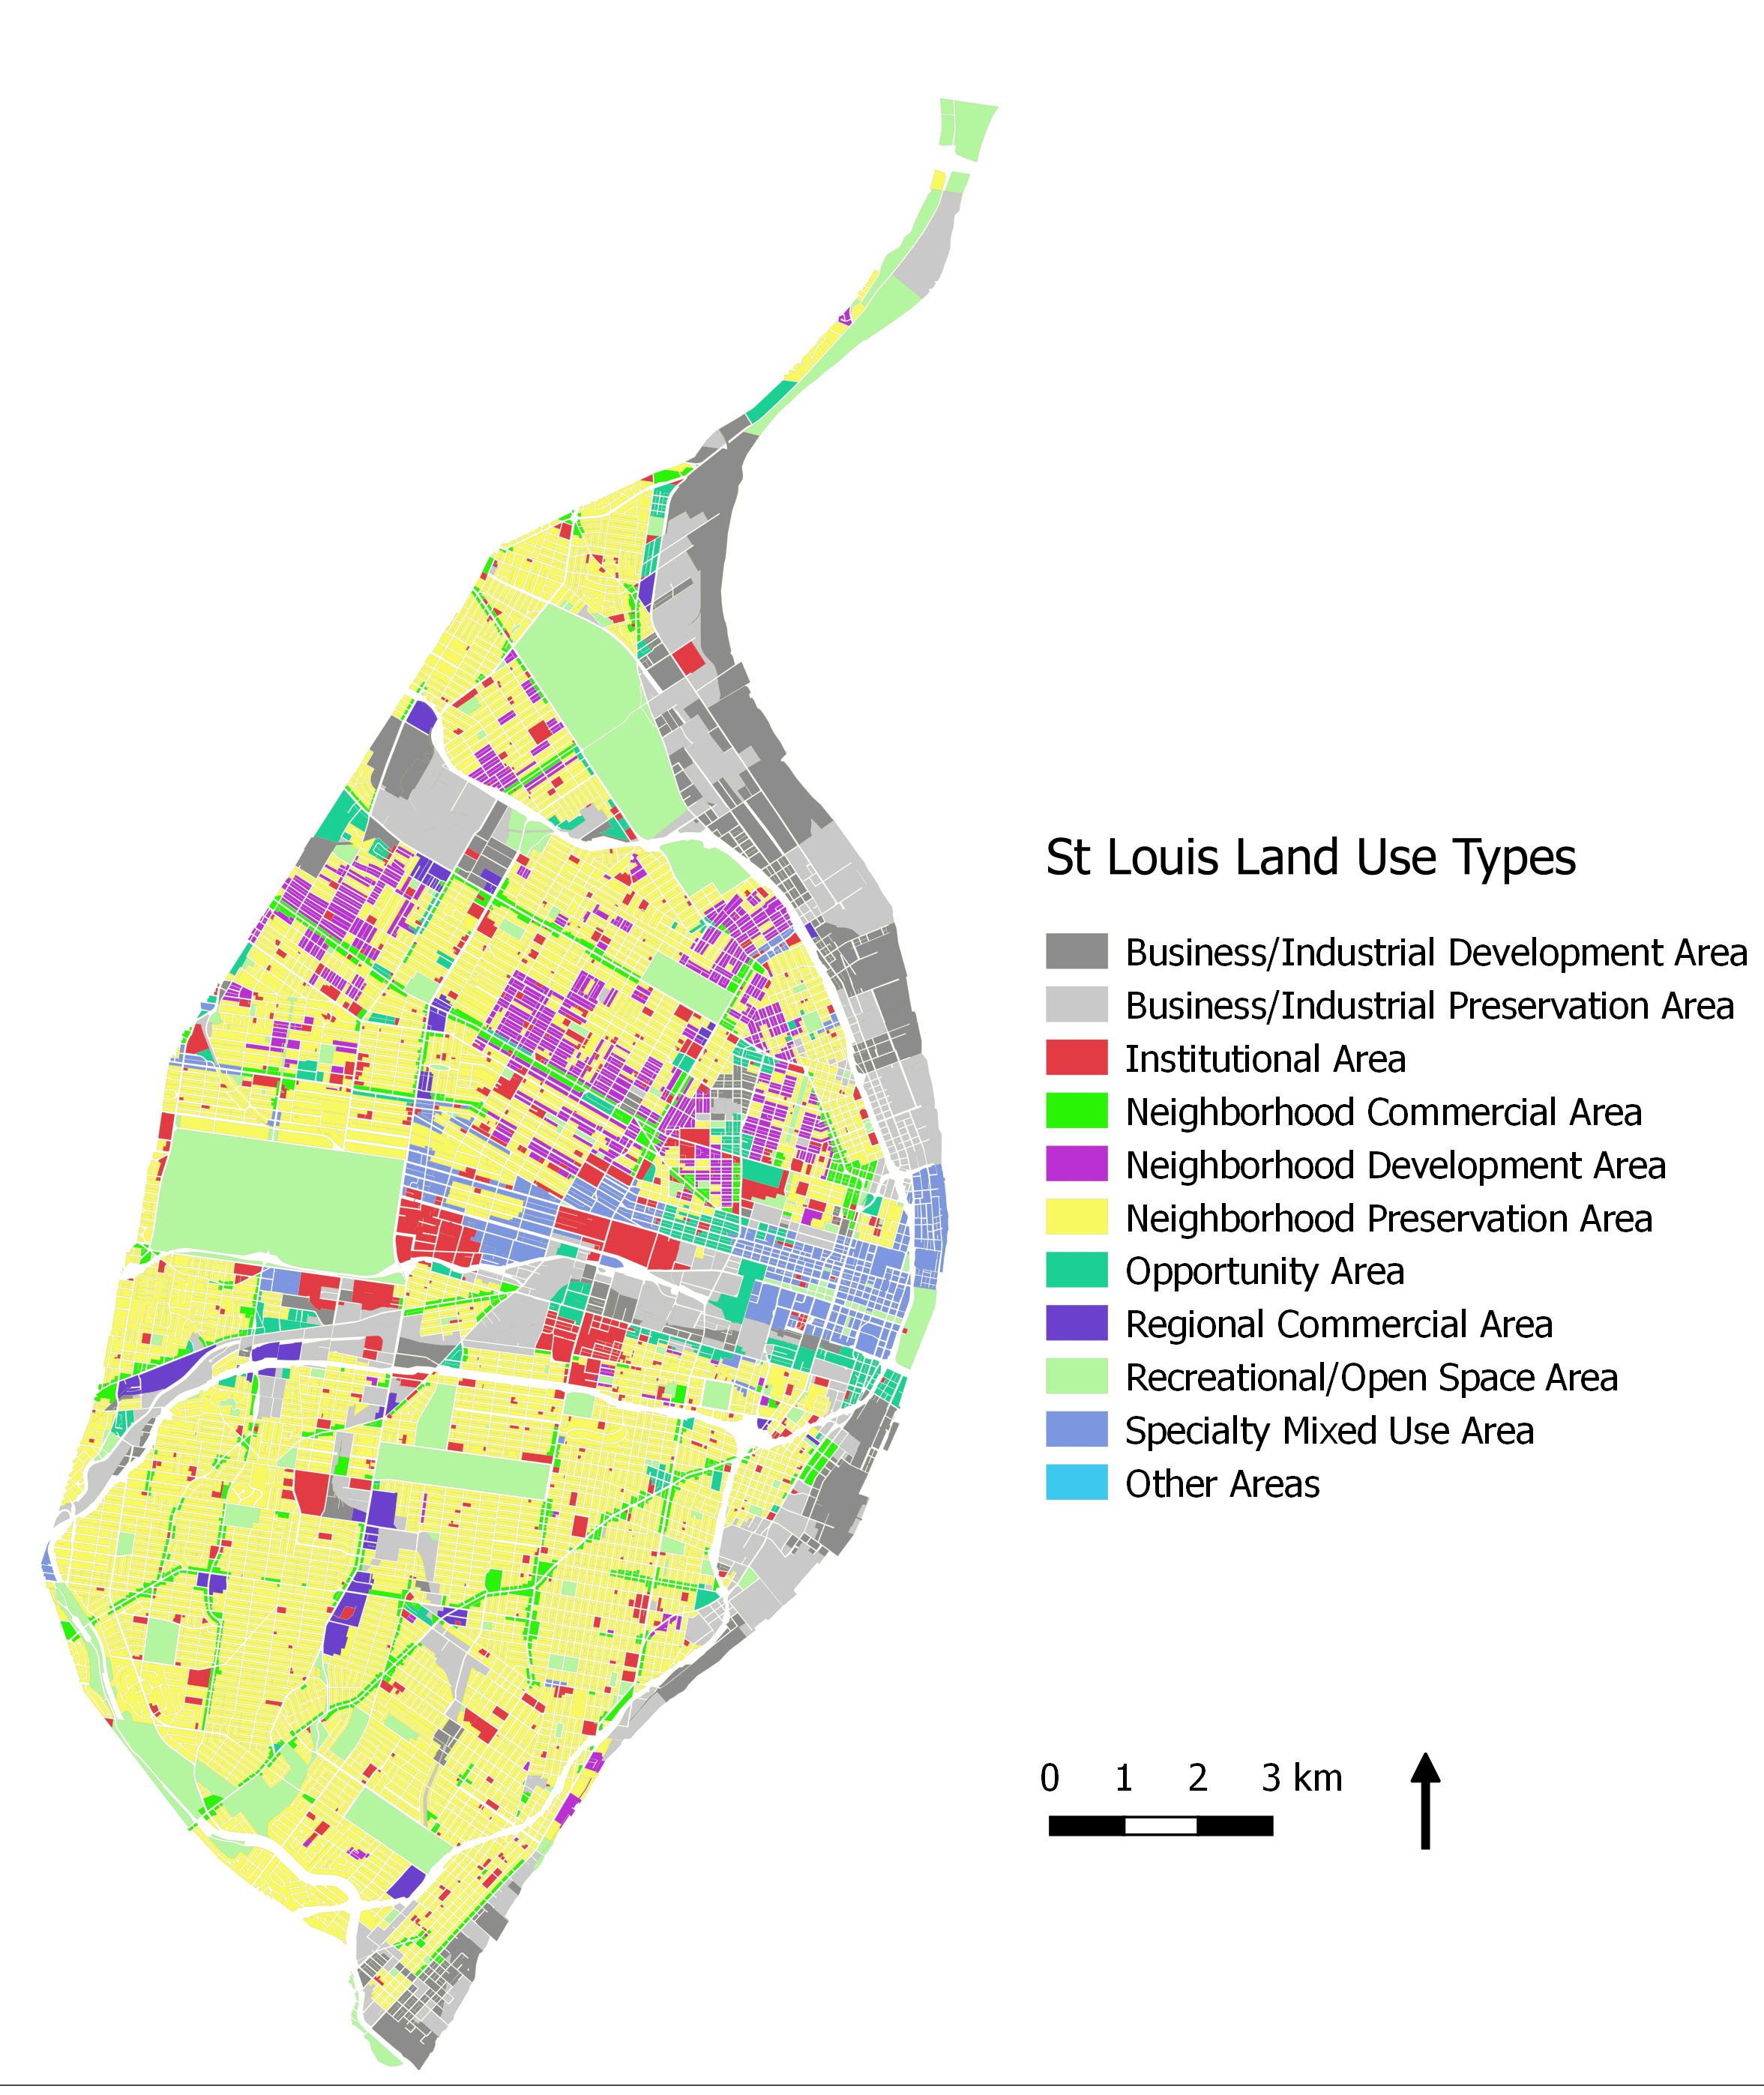
\includegraphics[width=\columnwidth]{fig1.png}}
\caption{St Louis Land Use Map}
\label{fig1}
\end{center}
\vskip -0.2in
\end{figure} 

If the number of tweets for a single user is too small, travel patterns could not be assessed. Therefore, we removed users with less than 10 tweets, and 237639 tweets of 2522 users were left in our experiment data-set. 

\subsubsection{Data Annotation}

We manually labeled these users with three gender types: male, female and others (including organizations and the uncertain), by investigating their profile images, first/last name and tweet contents. 

Usually, we do this task by the following order,

\begin{enumerate}
\item Check Twitter user avatar to judge whether user's gender.
\item Check Twitter account's first name.
\item Read tweet message history, to judge from the keywords in tweets like "father", "proud data", "my boyfriend", etc.
\item If still unclear, searching the user's first name, family name in Facebook, Instagram and Google+.
\item If still unclear, check the tweet message interaction between this user and his friends and using tweets like "I am proud of my friends and his girlfriend." to infer the gender.
\item if still unclear, we assign this user gender O which means others or unclear.
\end{enumerate}



\subsection{Feature Extraction}

In social media like Twitter, a user's tweet contains rich information about: where, when and what. We consider them as spatial features, temporal features and content features for further user gender identification. In this project, we focus on investigating relationships between users' travel patterns, tweet content and their gender affiliation. 

\subsubsection{Extract Temporal Feature}

We selected the following temporal features for each user  as candidate temporal features. Details are listed below,

\begin{enumerate}
\item Tweet frequency during 12 months (January to December)(12 features)
\item Tweet frequency during weekdays(Monday to Friday) or weekends(Saturday and Sunday).(2 features) 
\item Tweet frequency during different time period in one day and we allow overlapping between each time period. And each time period is determined as following using 24 hours(5 features): 
\begin{itemize}
\item Morning : 6:00 to 12:00
\item Noon : 11:00 to 14:00
\item Afternoon :  12:00 to 18:00 
\item Night :  17:00 to 23:00
\item Late-night :  22:00 to 6:00
\end{itemize}
\end{enumerate}

Using these features, we try to represent each Twitter users' temporal travel patterns.

\subsubsection{Extract Spatial Feature}

We selected the following spatial features for each user  as candidate spatial features. These features are using land use information to get the frequencies of tweets or the distance the Twitter user travel between each land type. Details are listed below,

\begin{enumerate}
\item Frequency of each zone type.(6 features)
\item Travel distance between every two different zone types on weekdays. (15 features)
\item Travel distance between every two different zone types on weekends. (15 features)
\end{enumerate}

Using these features, we try to represent each Twitter users' spatial l travel patterns.

\subsection{Extract Content Features}

We want to extract content features that can help identify different genders from each Twitter users' text content. Too many features will be used if we directly choose each word in tweet content. We have more than 10,000 unique word in all tweet content, this is overwhelmingly too large compared with spatial features and temporal features. Therefore, we applied naive Bayes network on the words of each user's tweet content and return confidences for different gender types.  Naive bayes network is a good model used for word classification due to its swiftness and simpleness \cite{cheng2010you,hansen2011good}. The network structure is illustrated in Fig. \ref{fig2}.

\begin{figure}[ht]
\vskip 0.2in
\begin{center}
\centerline{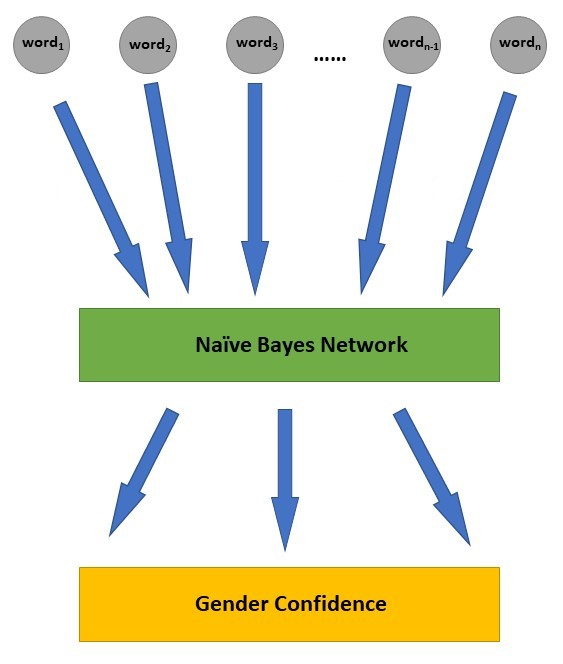
\includegraphics[width=\columnwidth]{fig2.jpg}}
\caption{Structure of Naive Bayes Network}
\label{fig2}
\end{center}
\vskip -0.2in
\end{figure} 

Naive Bayes network is based on Bayes Theorem which is shown in Fig. \ref{fig2}. It uses word embedding of each user tweet content to count the frequency of different word types existing in all instances in the train set and predicts the probability of Twitter users' genders, which called gender confidence in Fig. \ref{fig2}.

\subsection{Classification}

After getting gender confidence from naive Bayes network and combing this feature with 55 spatial and temporal features, we finally decided to use Random Forest to predict the final label of each user'  gender. Random Forest classification method was chosen because it could perform classification on high dimensional space by randomized feature selection approach\cite{breiman2001random}.  We have tested different methods based on our data, Random forest outperformed other methods like Neural network, Ada boosting and decision tree which agreed with other studies \cite{liaw2002classification}. In short, Random Forest is a form of "ensemble learning" where the algorithm generates a large number of not pruned decision trees and then summarize the results from each decision tree \cite{breiman2001random}. This means it can provide more accurate predictions with smaller sample sizes and becomes less susceptible to over-fitting and other problems in other classifiers. Therefore, we used the Random Forest functions \footnote{\url{http://scikit-learn.org/stable/modules/generated/sklearn.ensemble.RandomForestClassifier.html}} provided by Scikit-learn and trained the Random Forest classifier with 30 maximum features and 60 allowed sub-trees \cite{scikit-learn}.

\section{Results}
To better test our model and features, we randomly divide the whole data set into development data set(2400 users) and test data set(122 users). For the development stage, And we use 5-fold stratified cross validation to test our model for development stage. Specifically, the 2400 Twitter users are divided into development training set and development testing set. We use development testing set to help choose the best parameters for each model.

After we get the fully developed model, we use the test data set which is not used in development stage to test the accuracy of each model. And to better ensure the accuracy, we do the test of accuracy 5 times for each model. For each test Precision, Recall and F1-score are present.

\subsection{Accuracy} 

First, we present the accuracy result for content-based Naive Bayes Network as shown in Table. \ref{tab1} 

\begin{table}[tp]
\centering
\caption{Accuracy Table of Content-Based Naive Bayes Network}
\label{tab1}
\begin{center}
\begin{small}
\begin{sc}
\begin{tabular}{llll}
Experiment & Precision & Recall & F1-score \\ \hline
1          & 0.67      & 0.7    & 0.68     \\
2          & 0.72      & 0.73   & 0.72     \\
3          & 0.71      & 0.7    & 0.71     \\
4          & 0.72      & 0.72   & 0.72     \\
5          & 0.69      & 0.69   & 0.69     \\  \hline
Ave.       & 0.71      & 0.71   & 0.71   
\end{tabular}
\end{sc}
\end{small}
\end{center}
\end{table}

We can see that content-based Naive Bayes Network achieve an accuracy of 71 \%.

Secondly, we combine gender confidence given by naive Bayes network and travel pattern features to calculate Precision, Recall and F1-score again with different model.  All data are averaged 5 times.

\begin{table}[tp]
\centering
\caption{Performance Table of Combination of all feature with different models}
\label{tab2}
\begin{center}
\begin{small}
\begin{sc}
\begin{tabular}{llll}
Methods                    & Precision & Recall & F1-score \\ \hline
Random Forest              & \textbf{0.720}      & 0.725  & 0.720     \\
Decision Tree              & 0.715     & 0.733  & 0.723    \\
Extra Tree                 & 0.713     & 0.718  & 0.717    \\
AdaBoost Tree              & 0.718     & 0.725  & 0.718    \\
Gradient Boosting Tree     & 0.715     & 0.713  & 0.710     \\
Multi-layer Neural Network & 0.688     & 0.708  & 0.695   
\end{tabular}
\end{sc}
\end{small}
\end{center}
\end{table}


Apparently from Table. \ref{tab2},   we can find that,  after combining words and spatial and temporal features, precision, recall and F1-score increases for most models except multi-layer Neural Network which may need more parameter tuning before really achieving a good results.

To further test our method with the benchmark gender inference method using the first name as the vital feature for the inference and the result is shown in Table. \ref{tab3}.

\begin{table*}[tp]
\centering
\caption{Performance Table of Random Forest with all features and first name based methods}
\label{tab3}
\begin{center}
\begin{small}
\begin{sc}
\begin{tabular}{llll}
Methods                                     & Precision & Recall & F1-score \\
First name based                            & 0.898     & 0.785  & 0.832    \\
Random Forest with all features & 0.8230     & 0.835  & 0.830   
\end{tabular}
\end{sc}
\end{small}
\end{center}
\end{table*}

We can see that although our model is not better than benchmark method, the difference is small.  And out method does not require that first name must be provided by the user, which is helpful when first name is not provided or the field is not true. And we can see our method can be easily integrated with other methods.

\subsection{Spatial and Temporal Feature Importance}
As said above, our spatial and temporal feature are easily integrated with other methods, so here we want to show that adding spatial and temporal features can really improve the performance of both profile-based method(first name) and content-based methods. For this part, from the method above, we tried to  combine all spatial and temporal features with profile-based method and content-based method and output the relative importance of this feature in Random Forest. We only showed the top 10 important spatial and temporal features in Table. \ref{tab4} and Table. \ref{tab5}.

\begin{table}[tp]
\centering
\caption{Top 10 important spatial and temporal features for profile-based method(first name) }
\label{tab4}
\begin{center}
\begin{small}
\begin{sc}
\begin{tabular}{ll}
Feature Name & Importance \\ \hline
Confidence of gender M by first name & 0.3395		\\
Confidence of gender F by first name&  0.2683		\\
Confidence of gender O by first name&  0.0154 	\\
Frequency in May & 0.0195		\\
Frequency of stay at home & 0.0188 \\
Frequency on weekends & 0.0172		\\
Frequency at night &  0.0168		\\
Frequency at late night & 0.0167\\		
Frequency at afternoon & 0.0167	\\	
Frequency on weekdays & 0.0161		
\end{tabular}
\end{sc}
\end{small}
\end{center}
\end{table}


\begin{table}[tp]
\centering
\caption{Top 10 important spatial and temporal features for content-based method}
\label{tab5}
\begin{center}
\begin{small}
\begin{sc}
\begin{tabular}{ll}
Feature Name & Importance \\ \hline
Confidence of gender M by content & 0.4395 \\
Confidence of gender F by content & 0.2890 \\
Confidence of gender O by content & 0.0182 \\
Frequency on weekends& 0.0132 \\
Frequency at afternoon& 0.0120 \\
Frequency of stay at home&0.0119 \\
Frequency at night& 0.0109 \\
Frequency at late night&0.1082 \\
Frequency on weekdays&0.0094 \\
Frequency of commuting&0.0091 \\
\end{tabular}
\end{sc}
\end{small}
\end{center}
\end{table}

As is illustrated above, the confidences derived by first-name-based classifier or content based classifier contribute the most to gender classification. Aside from them, several spatial and temporal features were found to slightly improve the classification performance. They are frequency in May, frequency of stay at home, frequency on weekends, frequency at night, frequency at late night, frequency at afternoon, frequency on weekdays and frequency of commuting.

\subsection{Geo-Gender Map}
Due to time limit, we do not fully utilize the gender information we get for the Twitter users. However, here we show one usage of the obtained gender information in Fig. \ref{fig3}.

\begin{figure}[ht]
\vskip 0.2in
\begin{center}
\centerline{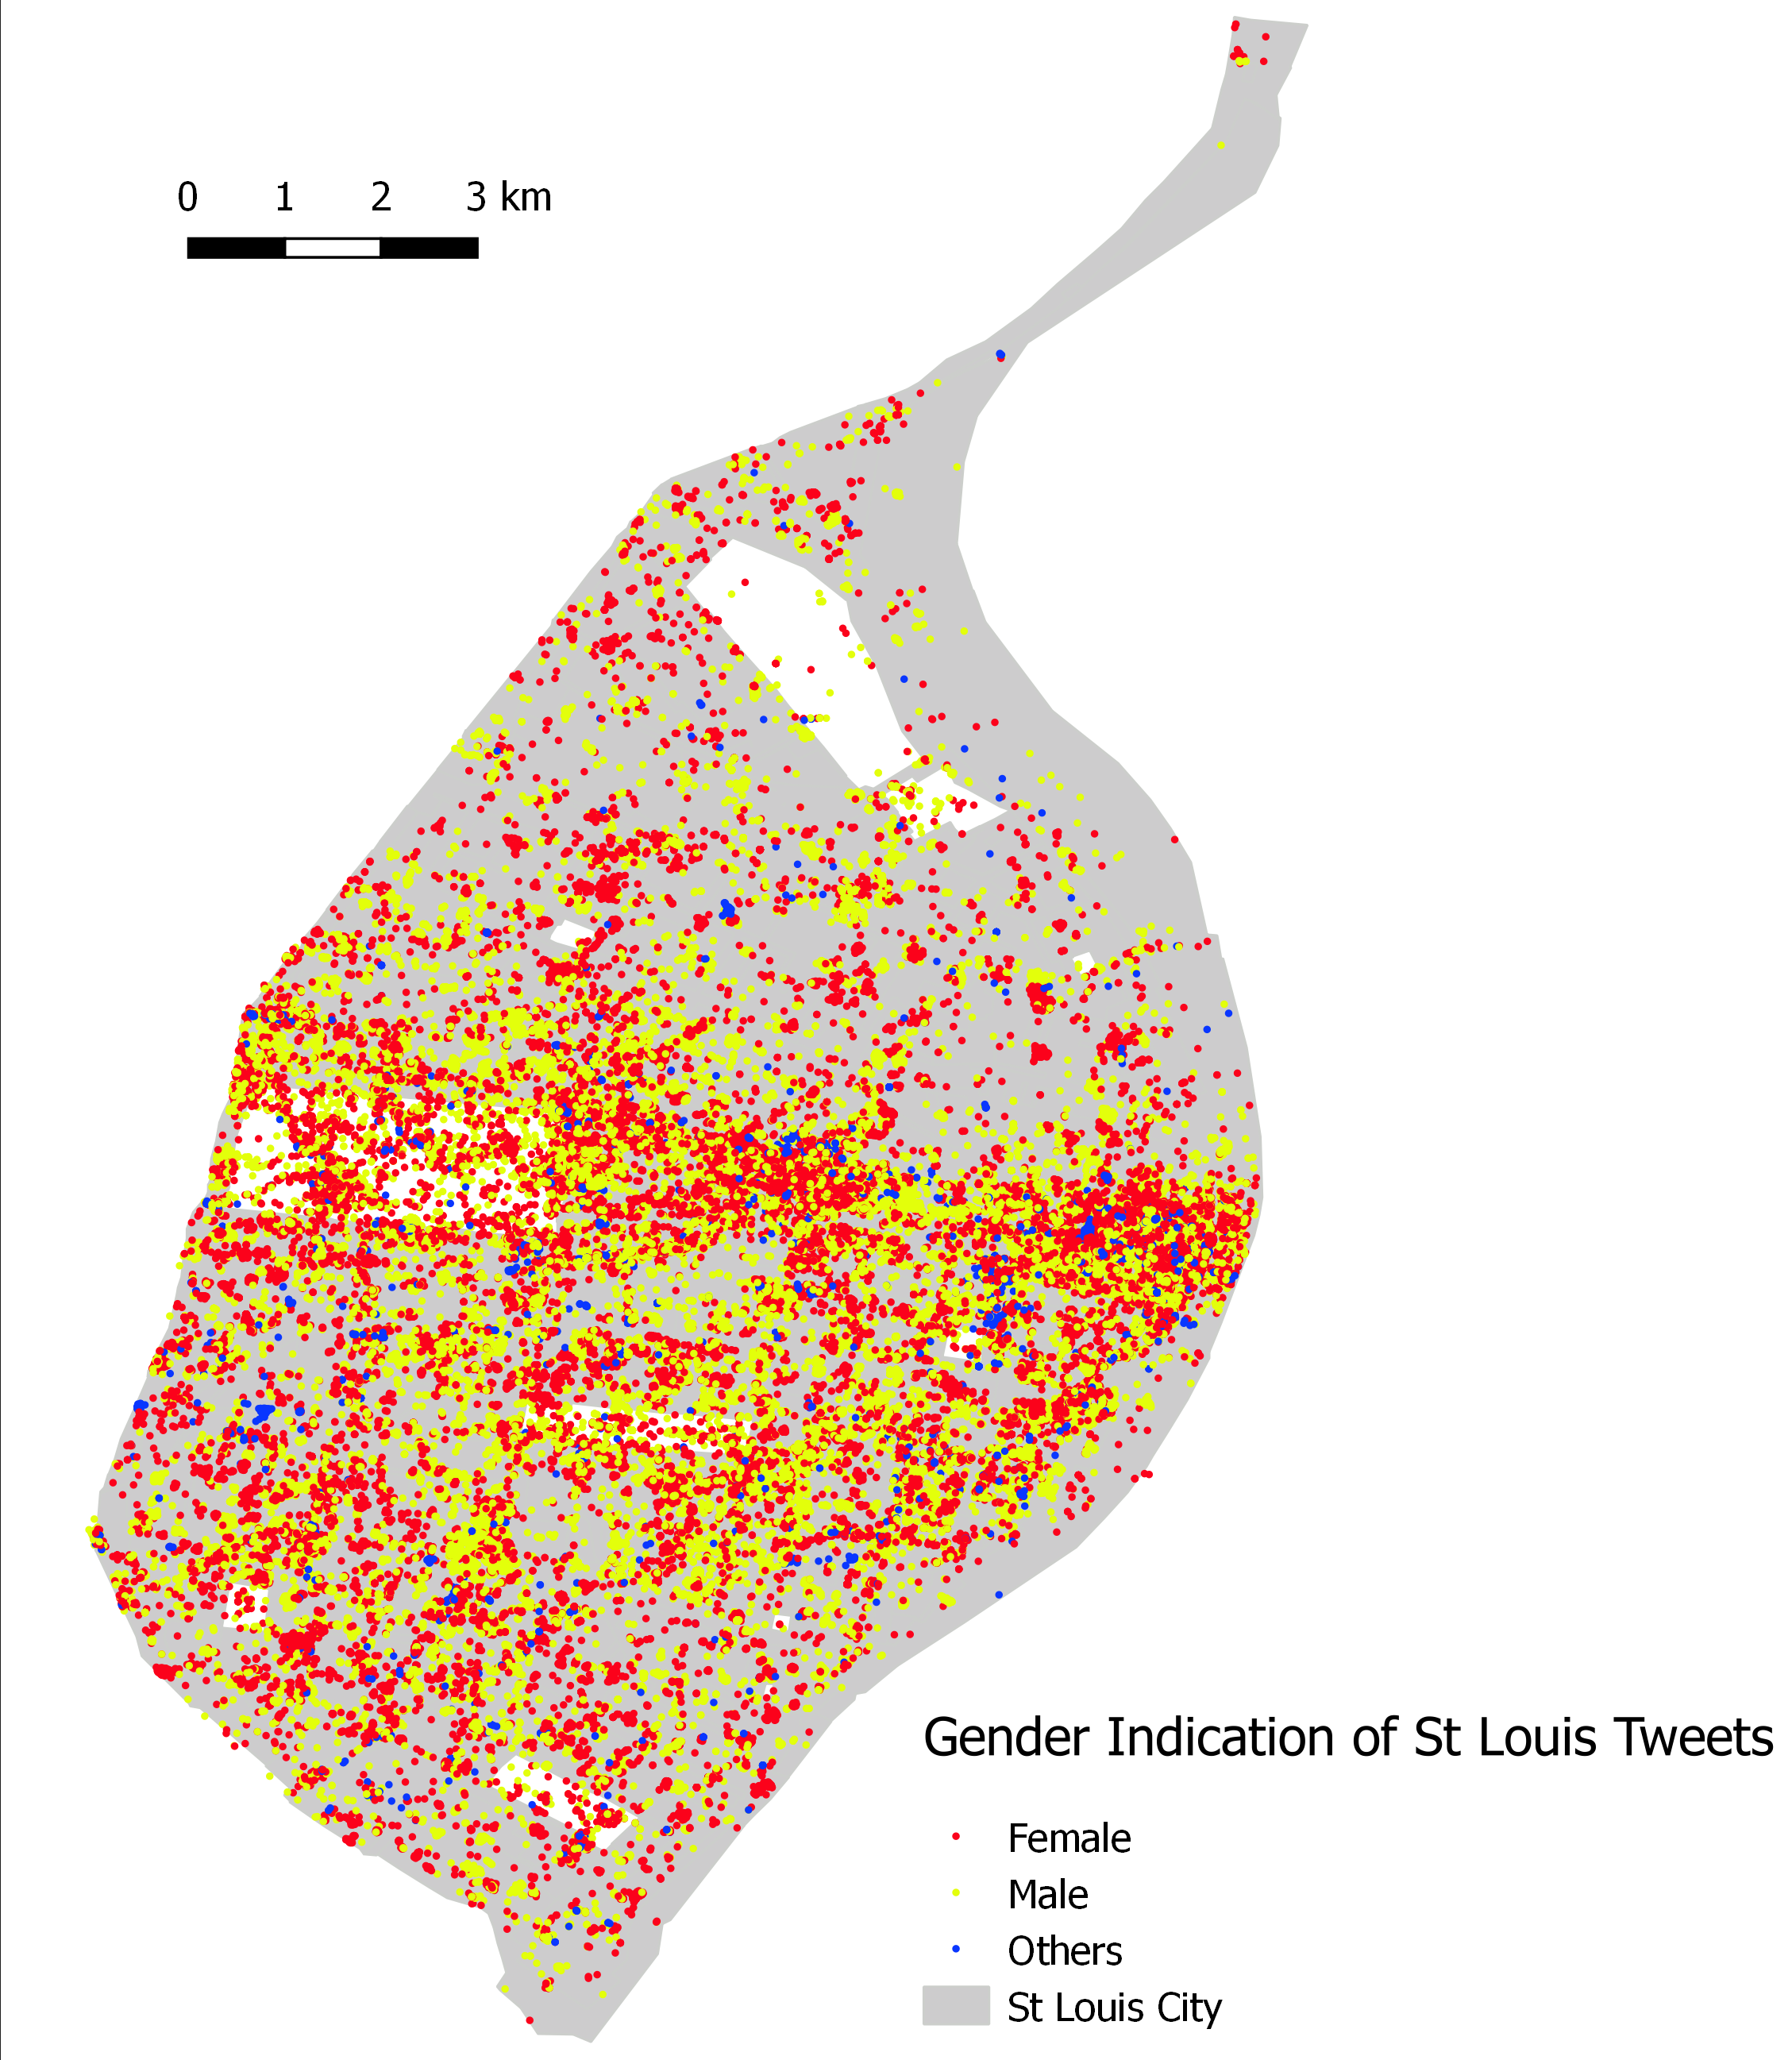
\includegraphics[width=\columnwidth]{fig3}}
\caption{Gender Geo-Distribution of St Louis Tweets}
\label{fig3}
\end{center}
\vskip -0.2in
\end{figure} 

Although it is hard to see any potential usage of  Fig. \ref{fig3}, it does show some gender features of St Louis which can be used by local government or  police department to  help the development of St Louis.

The final Random Forest model is shown in Appendix. 

\section{Discussion}

As shown in Table. \ref{tab2}, with the help of spatial and temporal features  to the content mining classifier, precision, recall and F1-score obviously increase under all the models except for Multi-layer Neural Network. We can conclude that travel pattern features works well and contribute positively to gender classification. As for the bad performance on Multi-layer Neural Network, it might result from that we did not acquire proper parameters for it. As shown in table 3, after adding spatial and temporal features to the first-name-based classifier, prediction recall gets clearly improved while the precision decreases. F1-scores of there two methods are nearly the same. It can be said that although our model does not predict as accurate as first name based model, we can get correct prediction within less attempt. And similar F1-scores indicted these two model have similar performance.


Compared with the gender classification based on users' first name, which generally gives a quite good result, our classification method shows a close performance. We cannot obtain users' first name correctly in some situations and it impedes the application of gender classification based on users' first name. However, we can get users' typical words from their contents quite conveniently and give a relatively high accuracy of gender classification with our model.

Word-embedding model is used in naive Bayes network, in which we count the frequency for different word types and construct a word table for that. With the word table we calculate different probabilities for gender types under the condition of these words and give gender confidences. However, one problem is that when classify tweet with the words out of the word table, something has to be done to include these words. To figure this problem we first extend the word table with the new words and then train the naive Bayes network again with the new word table. By using this method our word table becomes larger and larger and the chance to extend the word table becomes smaller and smaller. If the sample data set is large enough we will get a perfect dictionary for content classification. However, this needs more efforts on NLP related area.

\section{Conclusions}

Content method to process word content gives good results of gender classification of twitter users. Our model combines naive Bayes network and spatial and temporal features to predict Twitter user's gender. It further increases the performance of gender classification. Compared with users' first name gender classification, our model shows a close performance and has less restrictions in application.

In future, we will try to use larger data set with denser sampling of users' geographic locations. Then more accurate spatial and temporal features could be obtained and the performance of our model would be much further improved. 



%\begin{center}
%\textbf{\texttt{http://icml.cc/2017/}}
%\end{center}
%Send questions about submission and electronic templates to
%\texttt{icml2017pc@gmail.com}.
%
%The guidelines below will be enforced for initial submissions and
%camera-ready copies.  Here is a brief summary:
%\begin{itemize}
%\item Submissions must be in PDF.
%\item The maximum paper length is \textbf{8 pages excluding references and acknowledgements, and 10 pages
%  including references and acknowledgements} (pages 9 and 10 must contain only references and acknowledgements).
%\item Do \textbf{not include author information or acknowledgements} in your initial
%submission.
%\item Your paper should be in \textbf{10 point Times font}.
%\item Make sure your PDF file only uses Type-1 fonts.
%\item Place figure captions {\em under} the figure (and omit titles from inside
%the graphic file itself).  Place table captions {\em over} the table.
%\item References must include page numbers whenever possible and be as complete
%as possible.  Place multiple citations in chronological order.  
%\item Do not alter the style template; in particular, do not compress the paper
%format by reducing the vertical spaces.
%\item Keep your abstract brief and self-contained, one
%   paragraph and roughly 4--6 sentences.  Gross violations will require correction at the camera-ready phase.
%  Title should have content words capitalized.
%  
%
%\end{itemize}
%
%\subsection{Submitting Papers}
%
%{\bf Paper Deadline:} The deadline for paper submission to ICML 2017
%is at \textbf{23:59 Universal Time (3:59 p.m.\ Pacific Standard Time) on February 24, 2017}.
%If your full submission does not reach us by this time, it will 
%not be considered for publication. There is no separate abstract submission.
%
%{\bf Anonymous Submission:} To facilitate blind review, no identifying
%author information should appear on the title page or in the paper
%itself.  Section~\ref{author info} will explain the details of how to
%format this.
%
%{\bf Simultaneous Submission:} ICML will not accept any paper which,
%at the time of submission, is under review for another conference or
%has already been published. This policy also applies to papers that
%overlap substantially in technical content with conference papers
%under review or previously published. ICML submissions must not be
%submitted to other conferences during ICML's review period. Authors
%may submit to ICML substantially different versions of journal papers
%that are currently under review by the journal, but not yet accepted
%at the time of submission. Informal publications, such as technical
%reports or papers in workshop proceedings which do not appear in
%print, do not fall under these restrictions.
%
%\medskip
%
%To ensure our ability to print submissions, authors must provide their
%manuscripts in \textbf{PDF} format.  Furthermore, please make sure
%that files contain only Type-1 fonts (e.g.,~using the program {\tt
%  pdffonts} in linux or using File/DocumentProperties/Fonts in
%Acrobat).  Other fonts (like Type-3) might come from graphics files
%imported into the document.
%
%Authors using \textbf{Word} must convert their document to PDF.  Most
%of the latest versions of Word have the facility to do this
%automatically.  Submissions will not be accepted in Word format or any
%format other than PDF. Really. We're not joking. Don't send Word.
%
%Those who use \textbf{\LaTeX} to format their accepted papers need to pay close
%attention to the typefaces used.  Specifically, when producing the PDF by first
%converting the dvi output of \LaTeX\ to Postscript the default behavior is to
%use non-scalable Type-3 PostScript bitmap fonts to represent the standard
%\LaTeX\ fonts. The resulting document is difficult to read in electronic form;
%the type appears fuzzy. To avoid this problem, dvips must be instructed to use
%an alternative font map.  This can be achieved with the following two commands:
%
%{\footnotesize
%\begin{verbatim}
%dvips -Ppdf -tletter -G0 -o paper.ps paper.dvi
%ps2pdf paper.ps
%\end{verbatim}}
%Note that it is a zero following the ``-G''.  This tells dvips to use
%the config.pdf file (and this file refers to a better font mapping).
%
%A better alternative is to use the \textbf{pdflatex} program instead of
%straight \LaTeX. This program avoids the Type-3 font problem, however you must
%ensure that all of the fonts are embedded (use {\tt pdffonts}). If they are
%not, you need to configure pdflatex to use a font map file that specifies that
%the fonts be embedded. Also you should ensure that images are not downsampled
%or otherwise compressed in a lossy way.
%
%Note that the 2017 style files use the {\tt hyperref} package to
%make clickable links in documents.  If this causes problems for you,
%add {\tt nohyperref} as one of the options to the {\tt icml2017}
%usepackage statement.
%
%\subsection{Reacting to Reviews}
%
%We will continue the ICML tradition in which the authors are given the
%option of providing a short reaction to the initial reviews. These
%reactions will be taken into account in the discussion among the
%reviewers and area chairs.
%
%\subsection{Submitting Final Camera-Ready Copy}
%
%The final versions of papers accepted for publication should follow the
%same format and naming convention as initial submissions, except of
%course that the normal author information (names and affiliations)
%should be given.  See Section~\ref{final author} for details of how to
%format this.
%
%The footnote, ``Preliminary work.  Under review by the International
%Conference on Machine Learning (ICML).  Do not distribute.'' must be
%modified to ``\textit{Proceedings of the
%$\mathit{34}^{th}$ International Conference on Machine Learning},
%Sydney, Australia, PMLR 70, 2017.
%Copyright 2017 by the author(s).'' 
%
%For those using the \textbf{\LaTeX} style file, this change (and others) is
%handled automatically by simply changing
%$\mathtt{\backslash usepackage\{icml2017\}}$ to 
%$$\mathtt{\backslash usepackage[accepted]\{icml2017\}}$$
%Authors using \textbf{Word} must edit the
%footnote on the first page of the document themselves.
%
%Camera-ready copies should have the title of the paper as running head
%on each page except the first one.  The running title consists of a
%single line centered above a horizontal rule which is $1$ point thick.
%The running head should be centered, bold and in $9$ point type.  The
%rule should be $10$ points above the main text.  For those using the
%\textbf{\LaTeX} style file, the original title is automatically set as running
%head using the {\tt fancyhdr} package which is included in the ICML
%2017 style file package.  In case that the original title exceeds the
%size restrictions, a shorter form can be supplied by using
%
%\verb|\icmltitlerunning{...}|
%
%just before $\mathtt{\backslash begin\{document\}}$.
%Authors using \textbf{Word} must edit the header of the document themselves.
%
%\section{Format of the Paper} 
% 
%All submissions must follow the same format to ensure the printer can
%reproduce them without problems and to let readers more easily find
%the information that they desire.
%
%\subsection{Length and Dimensions}
%
%Papers must not exceed eight (8) pages, including all figures, tables,
%and appendices, but excluding references and acknowledgements. When references and acknowledgements are included,
%the paper must not exceed ten (10) pages.
%Acknowledgements should be limited to grants and people who contributed to the paper.
%Any submission that exceeds 
%this page limit or that diverges significantly from the format specified 
%herein will be rejected without review.
%
%The text of the paper should be formatted in two columns, with an
%overall width of 6.75 inches, height of 9.0 inches, and 0.25 inches
%between the columns. The left margin should be 0.75 inches and the top
%margin 1.0 inch (2.54~cm). The right and bottom margins will depend on
%whether you print on US letter or A4 paper, but all final versions
%must be produced for US letter size.
%
%The paper body should be set in 10~point type with a vertical spacing
%of 11~points. Please use Times typeface throughout the text.
%
%\subsection{Title}
%
%The paper title should be set in 14~point bold type and centered
%between two horizontal rules that are 1~point thick, with 1.0~inch
%between the top rule and the top edge of the page. Capitalize the
%first letter of content words and put the rest of the title in lower
%case.
%
%\subsection{Author Information for Submission}
%\label{author info}
%
%To facilitate blind review, author information must not appear.  If
%you are using \LaTeX\/ and the \texttt{icml2017.sty} file, you may use
%\verb+\icmlauthor{...}+ to specify authors and \verb+\icmlaffiliation{...}+ to specify affiliations. (Read the TeX code used to produce this document for an example usage.)  The author information
%will  not be printed unless {\tt accepted} is passed as an argument to the
%style file. (Again, see the TeX code used to produce this PDF.) 
%Submissions that include the author information will not
%be reviewed.
%
%\subsubsection{Self-Citations}
%
%If your are citing published papers for which you are an author, refer
%to yourself in the third person. In particular, do not use phrases
%that reveal your identity (e.g., ``in previous work \cite{langley00}, we 
%have shown \ldots'').
%
%Do not anonymize citations in the reference section by removing or
%blacking out author names. The only exception are manuscripts that are
%not yet published (e.g. under submission). If you choose to refer to
%such unpublished manuscripts \cite{anonymous}, anonymized copies have 
%to be submitted
%as Supplementary Material via CMT. However, keep in mind that an ICML
%paper should be self contained and should contain sufficient detail
%for the reviewers to evaluate the work. In particular, reviewers are
%not required to look a the Supplementary Material when writing their
%review.
%
%\subsubsection{Camera-Ready Author Information}
%\label{final author}
%
%If a paper is accepted, a final camera-ready copy must be prepared.
%%
%For camera-ready papers, author information should start 0.3~inches
%below the bottom rule surrounding the title. The authors' names should
%appear in 10~point bold type, in a row, separated by white space, and centered. 
%Author names should not be broken across lines.
%Unbolded superscripted numbers, starting 1, should be used to refer to affiliations. 
%Affiliations should be numbered in the order of appearance.  A single footnote block of text should be used to list all the affiliations. (Academic affiliations should list Department, University, City, State/Region, Country. Similarly for industrial affiliations.)
%Each distinct affiliations should be listed once.  If an author has multiple affiliations, multiple superscripts should be placed after the name, separated by thin spaces.  If the authors would like to highlight equal contribution by multiple first authors, those authors should have an asterisk placed after their name in superscript, and the term ``\textsuperscript{*}Equal contribution" should be placed in the footnote block ahead of the list of affiliations.  A list of corresponding authors and their emails (in the format Full Name \textless{}email@domain.com\textgreater{}) can follow the list of affiliations. Ideally only one or two names should be listed.
%
%
%A sample file (in PDF) with author names is included in the ICML2017 
%style file package.  Turn on the \texttt{[accepted]} option to the ICML stylefile to see the names rendered. 
%All of the guidelines above are automatically met by the \LaTeX\ style file.
%
%\subsection{Abstract}
%
%The paper abstract should begin in the left column, 0.4~inches below
%the final address. The heading `Abstract' should be centered, bold,
%and in 11~point type. The abstract body should use 10~point type, with
%a vertical spacing of 11~points, and should be indented 0.25~inches
%more than normal on left-hand and right-hand margins. Insert
%0.4~inches of blank space after the body. Keep your abstract brief and 
%self-contained,
%limiting it to one paragraph and roughly 4--6 sentences.  Gross violations will require correction at the camera-ready phase.
%
%\subsection{Partitioning the Text} 
%
%You should organize your paper into sections and paragraphs to help
%readers place a structure on the material and understand its
%contributions.
%
%\subsubsection{Sections and Subsections}
%
%Section headings should be numbered, flush left, and set in 11~pt bold
%type with the content words capitalized. Leave 0.25~inches of space
%before the heading and 0.15~inches after the heading.
%
%Similarly, subsection headings should be numbered, flush left, and set
%in 10~pt bold type with the content words capitalized. Leave
%0.2~inches of space before the heading and 0.13~inches afterward.
%
%Finally, subsubsection headings should be numbered, flush left, and
%set in 10~pt small caps with the content words capitalized. Leave
%0.18~inches of space before the heading and 0.1~inches after the
%heading. 
%
%Please use no more than three levels of headings.
%
%\subsubsection{Paragraphs and Footnotes}
%
%Within each section or subsection, you should further partition the
%paper into paragraphs. Do not indent the first line of a given
%paragraph, but insert a blank line between succeeding ones.
% 
%You can use footnotes\footnote{For the sake of readability, footnotes
%should be complete sentences.} to provide readers with additional
%information about a topic without interrupting the flow of the paper. 
%Indicate footnotes with a number in the text where the point is most
%relevant. Place the footnote in 9~point type at the bottom of the
%column in which it appears. Precede the first footnote in a column
%with a horizontal rule of 0.8~inches.\footnote{Multiple footnotes can
%appear in each column, in the same order as they appear in the text,
%but spread them across columns and pages if possible.}
%

%
%\subsection{Figures}
% 
%You may want to include figures in the paper to help readers visualize
%your approach and your results. Such artwork should be centered,
%legible, and separated from the text. Lines should be dark and at
%least 0.5~points thick for purposes of reproduction, and text should
%not appear on a gray background.
%
%Label all distinct components of each figure. If the figure takes the
%form of a graph, then give a name for each axis and include a legend
%that briefly describes each curve. Do not include a title inside the
%figure; instead, the caption should serve this function.
%
%Number figures sequentially, placing the figure number and caption
%{\it after\/} the graphics, with at least 0.1~inches of space before
%the caption and 0.1~inches after it, as in
%Figure~\ref{icml-historical}.  The figure caption should be set in
%9~point type and centered unless it runs two or more lines, in which
%case it should be flush left.  You may float figures to the top or
%bottom of a column, and you may set wide figures across both columns
%(use the environment {\tt figure*} in \LaTeX), but always place
%two-column figures at the top or bottom of the page.
%
%\subsection{Algorithms}
%
%If you are using \LaTeX, please use the ``algorithm'' and ``algorithmic'' 
%environments to format pseudocode. These require 
%the corresponding stylefiles, algorithm.sty and 
%algorithmic.sty, which are supplied with this package. 
%Algorithm~\ref{alg:example} shows an example. 
%
%\begin{algorithm}[tb]
%   \caption{Bubble Sort}
%   \label{alg:example}
%\begin{algorithmic}
%   \STATE {\bfseries Input:} data $x_i$, size $m$
%   \REPEAT
%   \STATE Initialize $noChange = true$.
%   \FOR{$i=1$ {\bfseries to} $m-1$}
%   \IF{$x_i > x_{i+1}$} 
%   \STATE Swap $x_i$ and $x_{i+1}$
%   \STATE $noChange = false$
%   \ENDIF
%   \ENDFOR
%   \UNTIL{$noChange$ is $true$}
%\end{algorithmic}
%\end{algorithm}
% 
%\subsection{Tables} 
% 
%You may also want to include tables that summarize material. Like 
%figures, these should be centered, legible, and numbered consecutively. 
%However, place the title {\it above\/} the table with at least 
%0.1~inches of space before the title and the same after it, as in 
%Table~\ref{sample-table}. The table title should be set in 9~point 
%type and centered unless it runs two or more lines, in which case it
%should be flush left.
%
%% Note use of \abovespace and \belowspace to get reasonable spacing 
%% above and below tabular lines. 
%

%
%Tables contain textual material that can be typeset, as contrasted 
%with figures, which contain graphical material that must be drawn. 
%Specify the contents of each row and column in the table's topmost
%row. Again, you may float tables to a column's top or bottom, and set
%wide tables across both columns, but place two-column tables at the
%top or bottom of the page.
% 
%\subsection{Citations and References} 
%
%Please use APA reference format regardless of your formatter
%or word processor. If you rely on the \LaTeX\/ bibliographic 
%facility, use {\tt natbib.sty} and {\tt icml2017.bst} 
%included in the style-file package to obtain this format.
%
%Citations within the text should include the authors' last names and
%year. If the authors' names are included in the sentence, place only
%the year in parentheses, for example when referencing Arthur Samuel's
%pioneering work \yrcite{Samuel59}. Otherwise place the entire
%reference in parentheses with the authors and year separated by a
%comma \cite{Samuel59}. List multiple references separated by
%semicolons \cite{kearns89,Samuel59,mitchell80}. Use the `et~al.'
%construct only for citations with three or more authors or after
%listing all authors to a publication in an earlier reference \cite{MachineLearningI}.
%
%Authors should cite their own work in the third person
%in the initial version of their paper submitted for blind review.
%Please refer to Section~\ref{author info} for detailed instructions on how to
%cite your own papers.
%
%Use an unnumbered first-level section heading for the references, and 
%use a hanging indent style, with the first line of the reference flush
%against the left margin and subsequent lines indented by 10 points. 
%The references at the end of this document give examples for journal
%articles \cite{Samuel59}, conference publications \cite{langley00}, book chapters \cite{Newell81}, books \cite{DudaHart2nd}, edited volumes \cite{MachineLearningI}, 
%technical reports \cite{mitchell80}, and dissertations \cite{kearns89}. 
%
%Alphabetize references by the surnames of the first authors, with
%single author entries preceding multiple author entries. Order
%references for the same authors by year of publication, with the
%earliest first. Make sure that each reference includes all relevant
%information (e.g., page numbers).



% Acknowledgements should only appear in the accepted version. 
\section*{Acknowledgements} 

We would like to sincerely thank Prof.Liang, Depratment of Computer Science at UW-Madison, for valuable suggestions to implement this project and Prof.Huang, Department of Geography at UW-Madison, for the help of collecting Twitter data-set and annotations of user genders.

\subsection*{Software and Data}

We provide all our data and program in Github and you can check them online \url{https://github.com/iphyer/cs760_TwitterDemographics}.

We use scikit-learn \cite{scikit-learn} as our machine learning program library and Pandas \cite{mckinney2015pandas} for data processing.

% In the unusual situation where you want a paper to appear in the
% references without citing it in the main text, use \nocite
%\nocite{langley00}

\bibliography{example_paper}
\bibliographystyle{icml2017}

\end{document} 


% This document was modified from the file originally made available by
% Pat Langley and Andrea Danyluk for ICML-2K. This version was
% created by Lise Getoor and Tobias Scheffer, it was slightly modified  
% from the 2010 version by Thorsten Joachims & Johannes Fuernkranz, 
% slightly modified from the 2009 version by Kiri Wagstaff and 
% Sam Roweis's 2008 version, which is slightly modified from 
% Prasad Tadepalli's 2007 version which is a lightly 
% changed version of the previous year's version by Andrew Moore, 
% which was in turn edited from those of Kristian Kersting and 
% Codrina Lauth. Alex Smola contributed to the algorithmic style files.  
